\section{}
\label{sec:problem3}
%%%%%%%%%%%%%%%%%%%%%%%%%%%%%%%%%%%%%%%%%%%%%%%%%%%%%%%%%%%%%%%%%%%%%%
In this exercise we consider the Neuman-Scott (Mother-Child) event RF model. Using this model the mother-model has a stationary Poisson RF with intensity $\lambda_M$. There exists $k^M$ mothers, and for each mother there exist a number of children, $k^c$, distributed according to a pdf $p(k^c)$ around the mother position $\vect{x}_j^M$, which is positionally distributed according to the conditional pdf $p(\vect{x} \given \vect{x}_j^M)$. The child position is then accepted to ensure that $\vect{x} \in \textrm{D}$. The set of samples generated from a Neuman-Scott event RF  is represented by
$\mathbb{X}_\textrm{D}^{NS}:\{\vect{x}_1,\vect{x}_2,...,\vect{x}_{k_\textrm{D}}\}:\{\vect{x}_{ji};j=1,2,...,k_\textrm{D}^M:i = 1,2,...,k_\textrm{D}^c\};\vect{x}_j,\vect{x}_{ji}\in D$ with the event count $k_\textrm{D} = \sum_j k_{\textrm{D}_j}^c$. The samples is generated from a sequential simulation algorithm given by

\begin{algorithm}[H]
\SetAlgoLined
initiate:\;
$k = 0$\;
$k^M \sim p(k) = Poi(k;\lambda_M) = \frac{[\lambda_M]^k}{k!}exp\{-\lambda_M\};k\in\mathbb{N}_\oplus$\;
\For{$j = 1,2,...,k^M$}{
Generate:\;
$\vect{x_j}\sim Uni[\textrm{D}]$\;
$k^c \sim p(k^c)$\;
\For{$i = 1,2,...,k^c$}{
Generate:\;
$\vect{x}^p\sim \phi_2(\vect{x};\vect{x}_j,\sigma_c^2\matr{I}_2)$\;

}
}
 \caption{How to write algorithms}
 \label{eq:SSNS}
\end{algorithm}
% \begin{equation}
%     \begin{array}{lll}
%         X_D^{NS} & \sim & p(\vect{x}_{ji}; j = 1,2,...,k_D^M; i =1,2,...,k_{D_j}^c) \\
%          & = & \prod\limits_{j=1}^{k_D^M}\left[\prod\limits_{i=1}^{k_{D_j}}\frac{ \vect{I}(\vect{x}_{ji}\in \mathrm{D})p(\vect{x}_{ji}\given\vect{x}_j^M)}{ P(\mathrm{D}\given\vect{x}_j^M)}\right]\times p(k_{D_j}^c\given k_j^c,\vect{x}_j^M)p(k_j^c)\times \frac{p(k_D^M)}{|D|^{k_D^M}} \\
%          & = & \prod\limits_{j=1}^{k_D^M}\left[\prod\limits_{i=1}^{k_{D_j}}\frac{ \vect{I}(\vect{x}_{ji}\in \mathrm{D}) \phi_2(\vect{x}_{ji};\vect{x}_j^M,\sigma_c^2\matr{I}_2)}{ \Phi_2(D;\vect{X}_j^M,\sigma_c^2\matr{I}_2 )}\right] \\
%          & \times & \Phi_2(D;\vect{x}_j^M,\sigma_c^2\matr{I}_2)^{k_{D_j}}[1-\Phi_2(\mathrm{D};\vect{x}_j^M,\sigma_c^2\matr{I}_2)]^{k_j^c-k_{D_j}^c}p(k_j^c)\\
%           & \times & \frac{[\lambda_M]^{k_D^M}}{k_D^M!}exp\{-\lambda_M|D|\};k_{D_j}^c\leq k_j^c
%          \end{array}
%     \label{eq:neumanscott}
% \end{equation}
From this we can see that the child position model is given by $\vect{x} \sim \Phi(\textrm{D};\vect{x}_j^M, \sigma_c^2\matr{I}_2)$. Then the model parameters are $\vect{\theta}_{pNS} = \left[\lambda_M,\sigma_c^2,p(\cdot)\right]$, where $\lambda_M$ is the intensity of the number of mothers, $\sigma_c^2$ is the deviation of the distance from a child to its mother, and $p(\cdot)$ is the distribution of the number of children around a mother.

To find the parameter $\lambda_M$ a cluster analysis is performed. We ran a gap statistic method for kmeans on the redwood tree data to determine the number of clusters or mothers. The result of which is shown in Figure \ref{fig:numb_clust}, giving $\lambda_M = 7$.

\begin{figure}
    \centering
    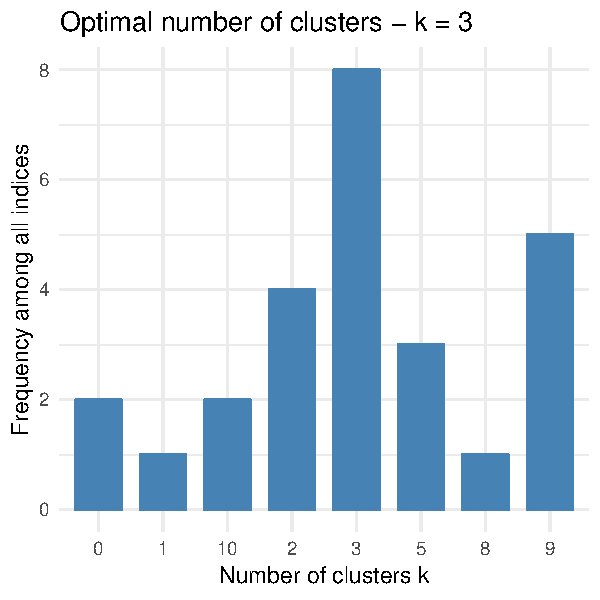
\includegraphics[scale=0.95]{figures/numb_clusters.pdf}
    \caption{Optimal number of cluster found using the gap statistics with kmeans of the redwood tree data.}
    \label{fig:numb_clust}
\end{figure}

To further analyze the redwood tree data a \textit{kmeans}-clustering is run to partition the data points as children in the $7$ clusters (mothers) found previously. The results are shown in Figure \ref{fig:cluster_part}. 

\begin{figure}
    \centering
    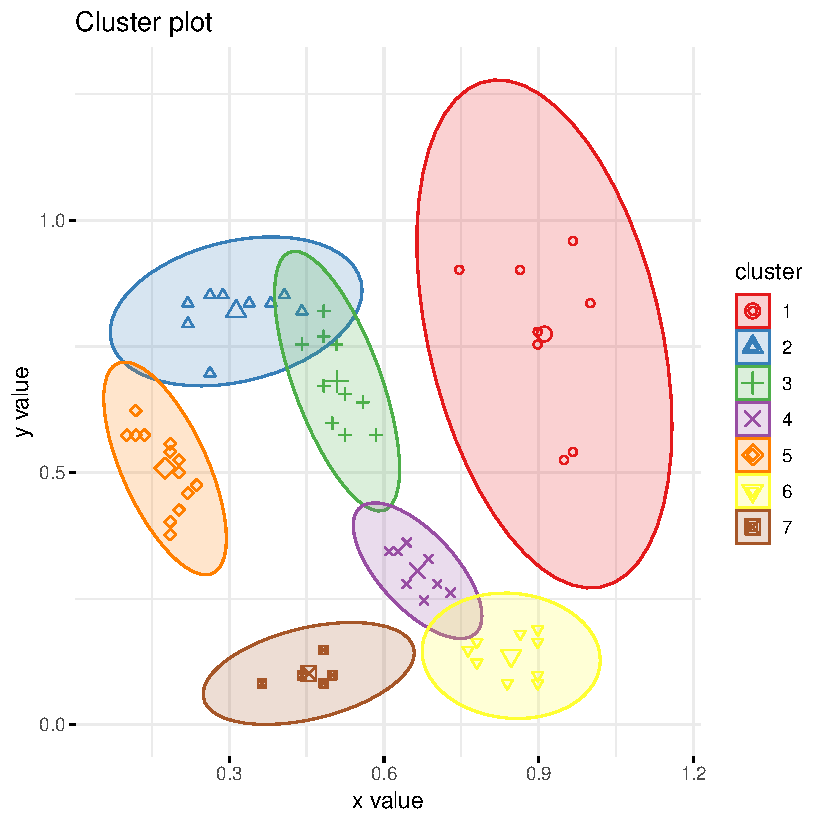
\includegraphics[scale=0.95]{figures/redwood_cluster_partitioning.pdf}
    \caption{Partition of children in cluster from the redwood tree data using kmean.}
    \label{fig:cluster_part}
\end{figure}

The distribution of number of children in a cluster, $p(\cdot)$, is chosen to be a binomial distribution. The maximum number of children in a cluster, is the number of data points in the redwood data $k_D$, and the probability of a child being child to the mother $k_j^M;j=1,2,...k^M$ is chosen to be $p(k_j^c \given k_j^M) = 1/k_j^M$. By this the number of children in a cluster is distributed as $k_j^c \sim \bin(k_D,1/k_j^M)$. For the positional distribution around the mother the parameter $\sigma_c^2$ is needed. This is given by the total sum of squares within a cluster $TSS; j\in 1,2,...,k^M$ and the number of children in a cluster $k_j^c$, s.t. $\sigma_c^2 = \mathrm{mean}(TSS/k_j^c)$.

Now we have all the model parameters. Next a simulation is run to find one realization of the Neuman-Scott event RF, shown in Figure \ref{fig:cluster_event_rf}.

\begin{figure}
    \centering
    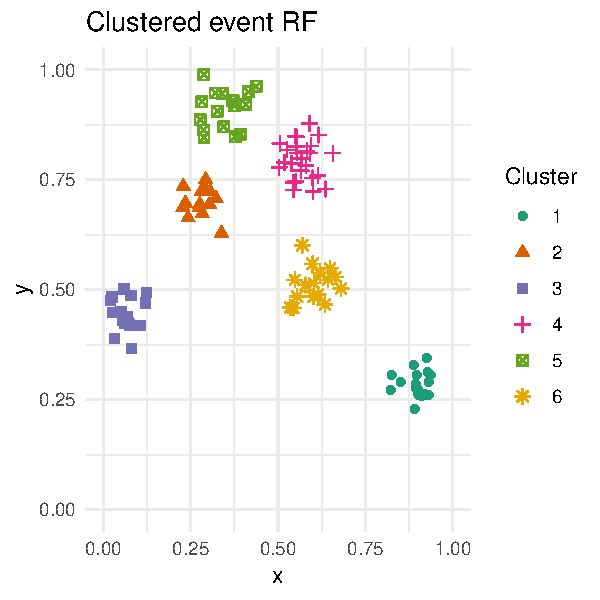
\includegraphics[scale=0.95]{figures/cluster_event_rf.pdf}
    \caption{One realization of a sequential simulation of a Neuman-Scott Event RF.}
    \label{fig:cluster_event_rf}
\end{figure}

Finally a Monte Carlo test is run on $100$ realizations from the Neuman-Scott event RF. The L-interaction function is calculated using Equation \eqref{eq:L_function} for each realization. The result is shown in Figure \ref{fig:gen_ns_l}.

\begin{figure}
    \centering
    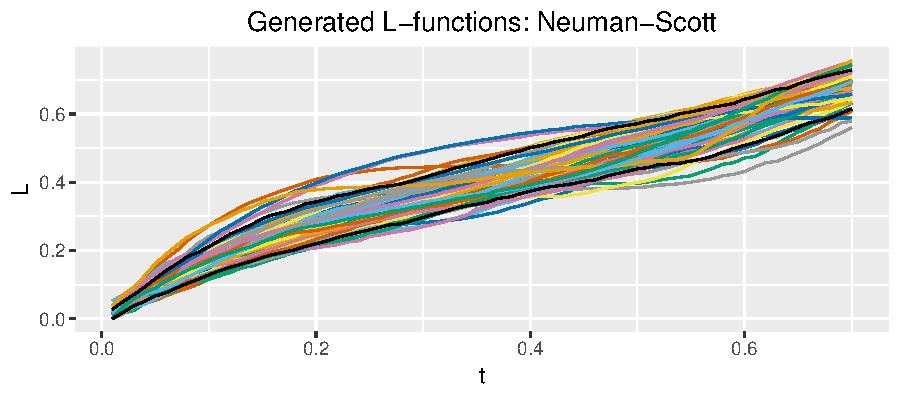
\includegraphics[scale=0.65]{figures/gen_ns_l.pdf}
    \caption{L-interaction function of $100$ realizations of a sequential simulation of a Neuman-Scott Event RF. The black lines is the $0.05$ and $0.95$ quantile of the L-interaction function.}
    \label{fig:gen_ns_l}
\end{figure}

\begin{figure}
    \centering
    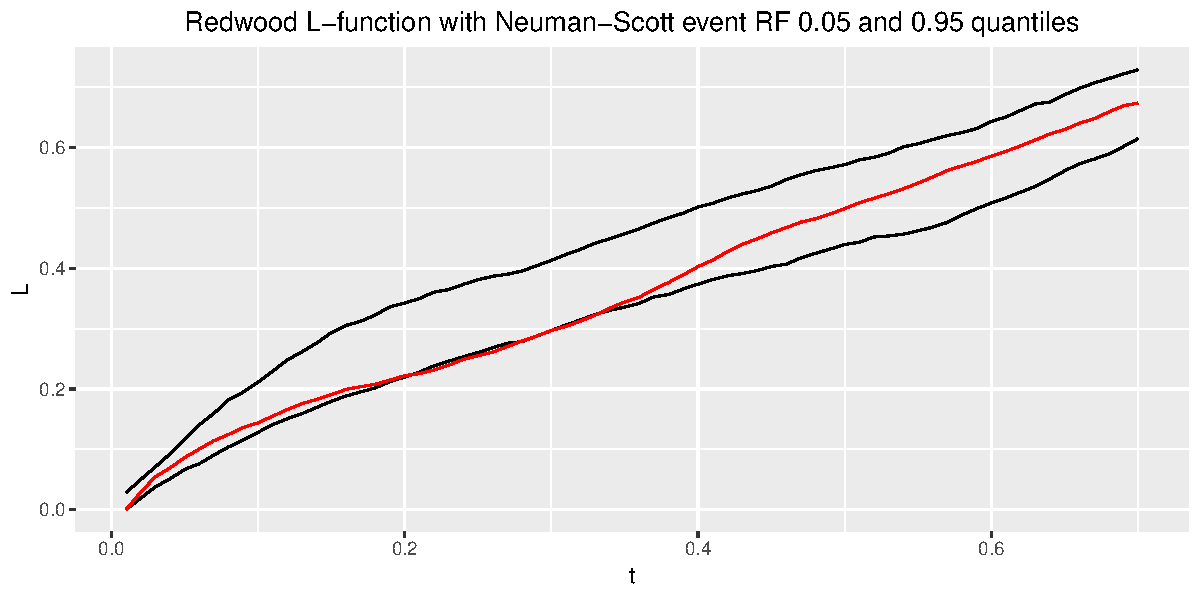
\includegraphics[scale=0.65]{figures/ns_quant1.pdf}
    \caption{A comparison between the $0.05$ and $0.95$ quantiles of the L-interaction function from $100$ realizations of a sequential simulation of a Neuman-Scott Event RF, and the L-interaction function of the redwood tree data.}
    \label{fig:ns_quant1}
\end{figure}

\begin{figure}
    \centering
    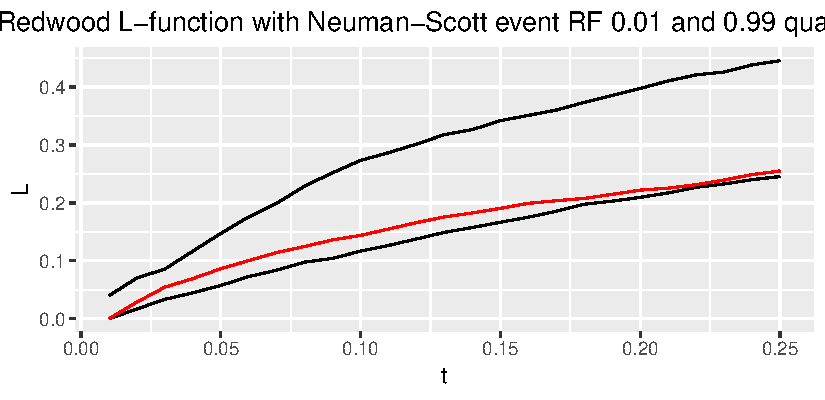
\includegraphics[scale=0.65]{figures/ns_quant2.pdf}
    \caption{A comparison between the $0.01$ and $0.99$ quantiles of the L-interaction function from $100$ realizations of a sequential simulation of a Neuman-Scot Event RF, and the L-interaction function of the redwood tree data.}
    \label{fig:ns_quant2}
\end{figure}

In Figure \ref{fig:ns_quant1} we see that the L-function of the redwood tree data lies between the $0.05$ and $0.95$ quantiles of the L-function of our realizations. The same conclusion can be drawn from Figure \ref{fig:ns_quant2} where the $0.01$ and $0.99$ quantiles are used. Which means that our model parameters fits the Neuman-Scott RF well to the redwood tree data. 